\documentclass[12pt,letterpaper]{article}
\usepackage{fullpage}
\usepackage[top=2cm, bottom=4.5cm, left=2.5cm, right=2.5cm]{geometry}
\usepackage{amsmath,amsthm,amsfonts,amssymb,amscd}
\usepackage{lastpage}
\usepackage{enumerate}
\usepackage{fancyhdr}
\usepackage{mathrsfs}
\usepackage{xcolor}
\usepackage{graphicx}
\usepackage{listings}
\usepackage{hyperref}
\usepackage{tikz-qtree}

\hypersetup{%
  colorlinks=true,
  linkcolor=blue,
  linkbordercolor={0 0 1}
}
 
\renewcommand\lstlistingname{Algorithm}
\renewcommand\lstlistlistingname{Algorithms}
\def\lstlistingautorefname{Alg.}

\lstdefinestyle{Python}{
    language        = Python,
    frame           = lines, 
    basicstyle      = \footnotesize,
    keywordstyle    = \color{blue},
    stringstyle     = \color{green},
    commentstyle    = \color{red}\ttfamily
}

\setlength{\parindent}{0.0in}
\setlength{\parskip}{0.05in}

% Edit these as appropriate
\newcommand\course{CSE 3500}
\newcommand\hwnumber{3}                  % <-- homework number
\newcommand\NetIDa{netid19823}           % <-- NetID of person #1

\pagestyle{fancyplain}
\headheight 35pt
\lhead{\NetIDa}
\chead{\textbf{\Large Homework \hwnumber}}
\rhead{\course \\ \today}
\lfoot{}
\cfoot{}
\rfoot{\small\thepage}
\headsep 1.5em

\tikzset{every tree node/.style={minimum width=2em,draw,circle},
         blank/.style={draw=none},
         edge from parent/.style=
         {draw,edge from parent path={(\tikzparentnode) -- (\tikzchildnode)}},
         level distance=1.5cm}

\begin{document}

\begin{center}
    \LARGE Problem Set
\end{center}


\section*{Problem 0 -- Dynamic Programming (25\%)}
Zoe starts at the top left corner of an $n \times n$ square grid of numbers and must end at the bottom right corner.
The numbers can be positive or negative. 
At each step, Zoe can go left, right, or down (but not up), and she can never revisit a square that she has already visited. 
Find an $O(n^2)$ algorithm to find the maximum sum of numbers Zoe can visit.\\

Given a $n \times n$ grid of numbers we can find the maximum sum of numbers Zoe can visit by finding 
the maximum numbers near the square from the top left corner to the bottom right corner and then adding the maximum sum of numbers.
Every square in the grid is grid[i][j] with i being the row and j being the column.
We can get the directions using grid[i-1][j] for down, grid[i][j-1] for left, and grid[i][j+1] for right.
We can then find the sum of the maximum numbers in a path by adding the current square to the maximum of the three directions
which is grid[i][j] + max(grid[i-1][j], grid[i][j-1], grid[i][j+1]). 
If we do this for every square in the grid we can now compare each value and formulate a path from that and find the maximum sum of numbers Zoe can visit that leads to the bottom right corner.
The algorithm is $O(n^2)$ because we have to go through every square in the grid.
We use 2 for loops to go through every square in the grid and we use 3 if statements to find the maximum of the three directions.

\newpage

\section*{Problem 1 -- Divide and Conquer (25\%)}
A mad scientist accidentally left her cloning machine on and open while vacationing in Storrs, Connecticut.
While she was away, a murder of crows managed to get inside her office and use the cloning machine.
The mad scientist returned from her vacation surprised to have her office full of crows, but excited to test a new hypothesis.
As is well known, crows are very intelligent birds, and the scientist suspects that one or more crows may have taken advantage of the cloning machine to gain a selective genetic advantage.

We say that two crows are \textit{identical} if we genetically sequence the crows and their DNA is 99.99\% identical.
The mad scientist has a machine that will determine whether or not two crows are genetically identical, but it is costly to operate so she wants to minimize its use.

The only operation you are allowed to perform is to take two crows and determine if they are genetically identical.
Develop an $O(n \log n)$ algorithm that, given $n$ crows, determines if there is a set of more than $n/2$ crows that are genetically identical.
\\[14pt]
For this problem we can use a form of divide and conquer. 
We can visualize the crows as a list of numbers, with 
each number representing a unique crow and the same number representing the same/clone crow.
We would then split the list in half over and over until we have a list of size 1 crow.
From that we then start conquering the list back up and merge the lists together.
When we go up and merge the lists the first time, we would be comparing only 2 crows.
On that level we compare all the groups of 2 crows and if we find a match we consider that a majority.
If there is no match then we don't consider that a majority. We then move up a level
which combines the groups of 2 crows into groups of 4 crows and compare all the groups of 4 crows.
If one of the joined groups had a majority and one is not then we compare the majority element to the other elements to find out if there is a majority.
If the majority group is paired with another majority group of a diffrent element then we don't consider that a majority.
If we do this for every level we can find the set of more than $n/2$ crows in $O(n \log n)$ time.
We compare each level of crows in $O(n)$ time and we have to do this for $O(\log n)$ levels.


\newpage

\section*{Problem 2 -- SillySort (25\%)}

Prove that SillySort(L) terminates and correctly sorts its input list of numbers $L$.

    \lstset{caption={A sorting algorithm only used by silly people.}}
    \lstset{label={lst:alg1}}
     \begin{lstlisting}[style = Python]
    def sillysort(L):
        while true:
            if L is sorted:
                return L
            else:
                compute an arbitrary index i such that L[i] > L[i+1]
                swap L[i] and L[i+1]
    \end{lstlisting}

SillySort's end condition is that the list is sorted.
It will continue to run and swap the numbers until the list is sorted.
The algorithm acts similar to bubble sort as it also swaps two indexes until the list is sorted.
The worst case scenario for SillySort is that the list is in reverse order
as it will have to swap every index all the way to the end of the list to sort it.
The best case scenario for SillySort is that the list is already sorted as it will not have to swap any indexes.
The average case scenario for SillySort is that the list is in random order as it will have to swap some indexes to sort the list.
We can also assume that by "compute an arbitrary index i such that $L[i] > L[i+1]$" 
that the algorithm will find the indexes that satisfy $L[i] > L[i+1]$ and skip over those that are already sorted.
The time complexity for SillySort is $O(n^2)$ as it will
have to iterate through the list $n$ times and swap the indexes $n$ times.
The space complexity for SillySort is $O(1)$ as it will not use any extra space.
We can test the correctness of SillySort by using a list of numbers and sorting it.
We can first use $L = [1, 2, 3, 4, 5]$ which is a already sorted list. If we
pass this list into SillySort it will return the same list as it is already sorted.
We can then use $L = [2, 1, 3, 5, 4]$ which is a list in random order. If we
pass this list into SillySort it would run the algorithm multiple times until the list is sorted.
We can give SillySort a arbitrary value for $i$ that satisfies $L[i] > L[i+1]$ 
like $i = 0$. This will swap the values at index 0 and 1 which are 2 and 1 respectively.
The new list would be $L = [1, 2, 3, 5, 4]$. We can then give another arbitrary value for $i$ 
which only one index satisfies $L[i] > L[i+1]$ which is $i = 3$. This will swap the values at index 3 and 4
which are 5 and 4 respectively. The new list would be $L = [1, 2, 3, 4, 5]$. This list is now sorted and
SillySort will return the list. Given that SillySort could swap the indexes multiple times until the list is sorted,
we can infer that SillySort can be and correctly used on any list of numbers. The worst case scenario for SillySort
is that the list is in reverse order as it will have to swap every index all the way to the end of the list to sort it.
An example of this would be $L = [5, 4, 3, 2, 1]$. If we pass this list into SillySort it would run the algorithm
like we did before, it would return $L = [1, 2, 3, 4, 5]$ which is the sorted list. 
This means that SillySort will correctly sort any list of numbers.

\newpage

\section*{Problem 3 -- Data structures (25\%)}

\begin{enumerate}
    \item We saw in class the algorithm for building a max-heap

    \lstset{caption={Building a max heap.}}
    \lstset{label={lst:alg1}}
     \begin{lstlisting}[style = Python]
    import math
    def buildmaxheap(A):
        A.heapsize = A.length
        for i in range(int(math.floor(A.length/2)),0,-1):
            maxheapify(A,i)
    \end{lstlisting}

Consider the following alternative way to build a max-heap

    \lstset{caption={Building a max heap.}}
    \lstset{label={lst:alg1}}
     \begin{lstlisting}[style = Python]
    def buildmaxheap2(A):
        A.heapsize = 1
        for i in range(2,A.length+1):
            maxheapinsert(A,A[i])
    \end{lstlisting}

Prove that buildmaxheap and buildmaxheap2 do not always create the same heap by providing a counterexample.
\\[14pt]
Given both buildmaxheap and buildmaxheap2, they do 
not always create the same heap. A example of this would be 
making a max heap of $[1,2,3]$. The first algorithm, buildmaxheap,
would create a max heap of $[3,2,1]$. The second algorithm, buildmaxheap2,
would create a max heap of $[3,1,2]$.\\
\begin{center}
    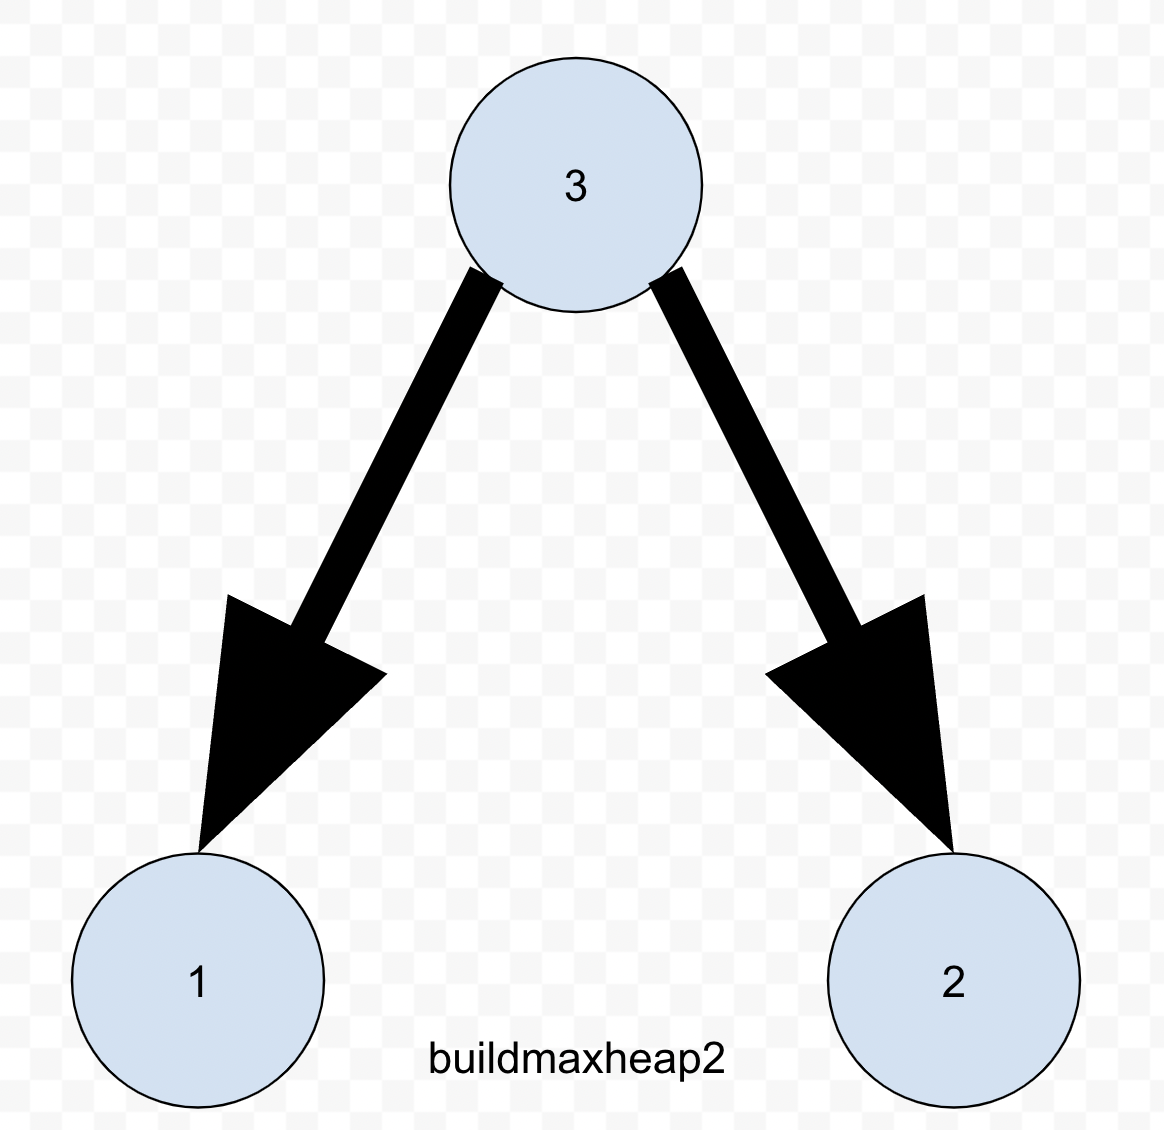
\includegraphics[scale=.25]{images/buildmaxheap.png}
    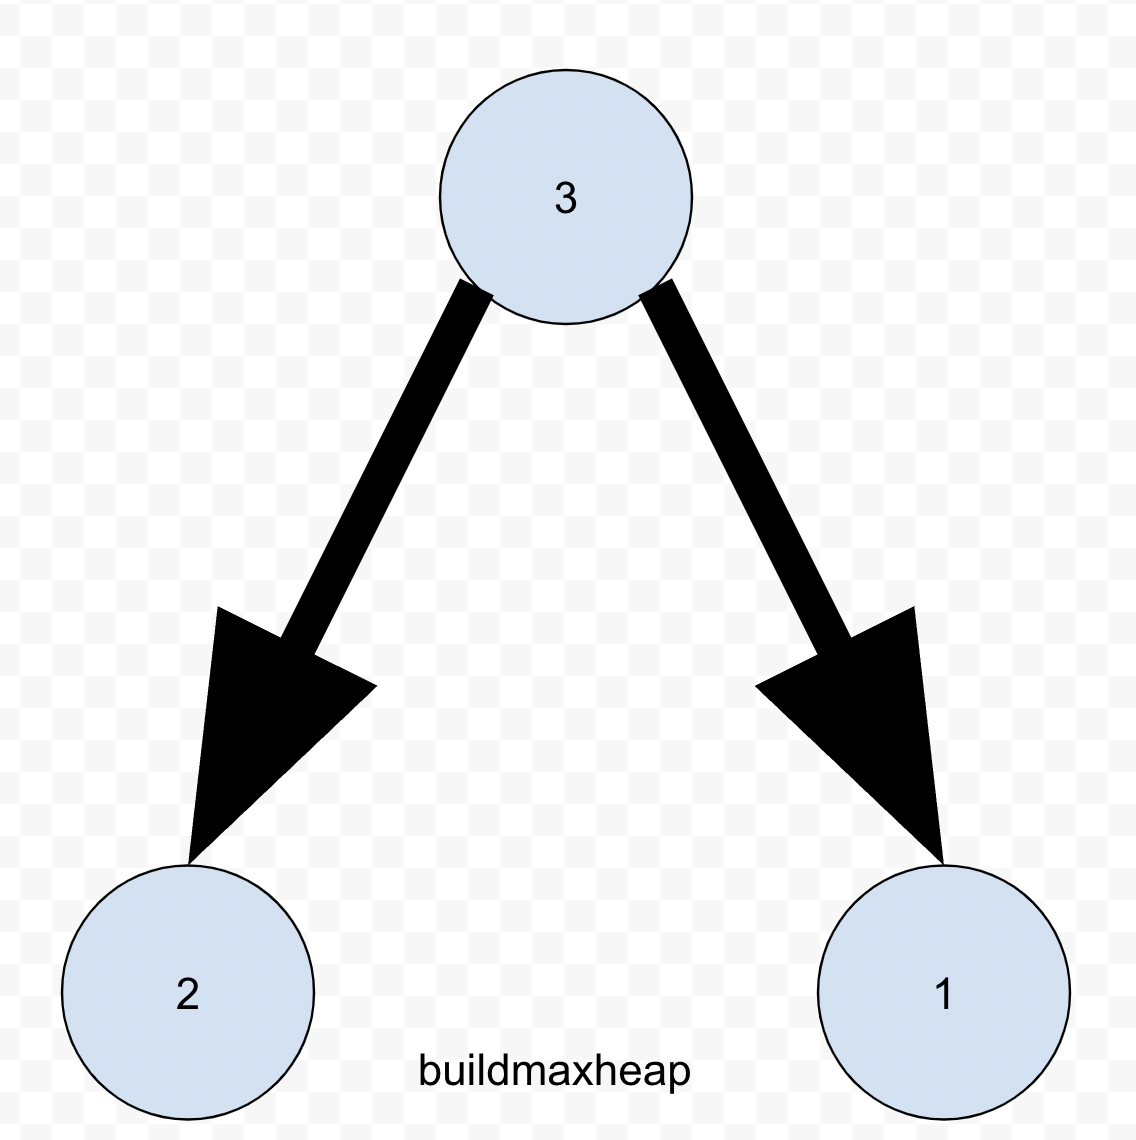
\includegraphics[scale=.25]{images/buildmaxheap2.png}
\end{center}
    \item What is the worst case time complexity of buildmaxheap2? Explain your reasoning.
    \\[14pt]
    The worst case time complexity of buildmaxheap2 is $O(n \log n)$.
    This is because the algorithm will have to iterate through the list $n$ times
    and call maxheapinsert which has a time complexity of $O(\log n)$.
    Therefore, the time complexity of buildmaxheap2 is $O(n \log n)$.

\end{enumerate}




\end{document}
